\documentclass[tikz,border=8pt]{standalone}
\usetikzlibrary{arrows.meta,calc}

\begin{document}
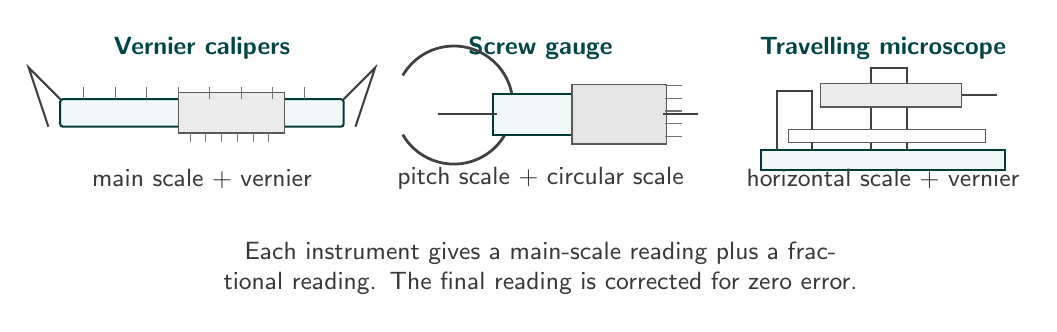
\begin{tikzpicture}[
  line/.style={draw=black!75,line width=0.75pt},
  soft/.style={draw=teal!45!black,fill=teal!6,line width=0.75pt},
  label/.style={font=\sffamily\small,text=black!78},
  title/.style={font=\sffamily\bfseries\small,text=teal!55!black},
]

% Vernier caliper panel
\node[title] at (-4.3,2.9) {Vernier calipers};
\draw[soft,rounded corners=1pt] (-6.1,1.9) rectangle (-2.5,2.25);
\draw[line] (-6.1,2.25) -- (-6.5,2.65) -- (-6.25,1.9);
\draw[line] (-2.5,2.25) -- (-2.1,2.65) -- (-2.35,1.9);
\draw[fill=black!8,draw=black!65] (-4.6,1.82) rectangle (-3.25,2.34);
\foreach \x in {-5.8,-5.4,...,-2.8}
  \draw[black!55] (\x,2.25) -- ++(0,0.16);
\foreach \x in {-4.45,-4.25,...,-3.45}
  \draw[black!55] (\x,1.82) -- ++(0,-0.12);
\node[label] at (-4.3,1.24) {main scale + vernier};

% Screw gauge panel
\node[title] at (0,2.9) {Screw gauge};
\draw[line,line width=1pt] (-1.75,1.8) arc[start angle=210,end angle=510,radius=0.75];
\draw[soft] (-0.6,1.8) rectangle (0.4,2.32);
\draw[fill=black!10,draw=black!65] (0.4,1.68) rectangle (1.6,2.44);
\draw[line] (-1.3,2.06) -- (-0.55,2.06);
\draw[line] (1.55,2.06) -- (2.0,2.06);
\foreach \y in {1.78,1.94,2.10,2.26,2.42}
  \draw[black!55] (1.58,\y) -- ++(0.22,0);
\node[label] at (0,1.24) {pitch scale + circular scale};

% Travelling microscope panel
\node[title] at (4.35,2.9) {Travelling microscope};
\draw[soft] (2.8,1.35) rectangle (5.9,1.6);
\draw[line] (3.0,1.6) -- (3.0,2.35) -- (3.45,2.35) -- (3.45,1.6);
\draw[line] (4.2,1.6) -- (4.2,2.65) -- (4.65,2.65) -- (4.65,1.6);
\draw[fill=black!8,draw=black!65] (3.55,2.15) rectangle (5.35,2.45);
\draw[line] (5.35,2.30) -- (5.8,2.30);
\draw[fill=white,draw=black!65] (3.15,1.7) rectangle (5.65,1.86);
\node[label] at (4.35,1.24) {horizontal scale + vernier};

\node[label,align=center,text width=11.4cm] at (0,0.1)
  {Each instrument gives a main-scale reading plus a fractional reading. The final reading is corrected for zero error.};

\end{tikzpicture}
\end{document}
